%% Figure: oracle frequency in the 49 main-corpus papers (mapping/4_coding/coding.csv;
%% mapping/analysis/recompute.py prints the same numbers).
%% A paper can use several oracles, so bars do not sum to 49.
%% To change a number, edit both the bar value and its label [n (p%)].
%% Revised 26 Oct 2026 after review: TRAVEL, PtrTrans, ReCodeAgent and MBTA
%% recoded, and CAST gains O-b under the compilation rule (option B);
%% bars sorted by count again.
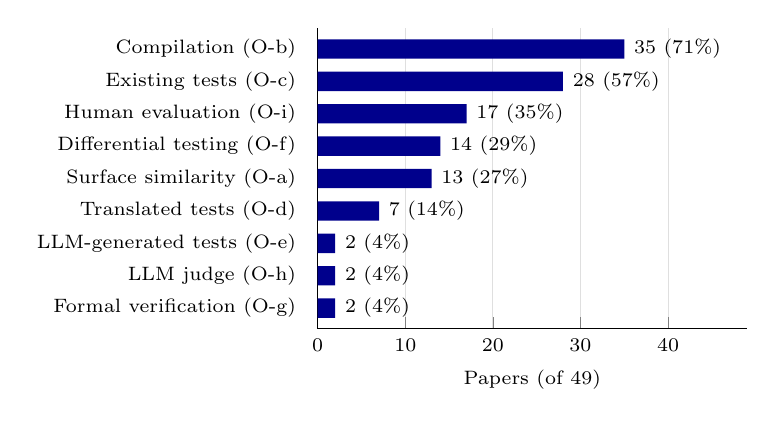
\begin{tikzpicture}
\begin{axis}[
  xbar, width=0.58\columnwidth, height=5.4cm, xmin=0, xmax=49, y dir=reverse,
  ytick=data, symbolic y coords={ob,oc,oi,of,oa,od,oe,oh,og},
  yticklabels={{Compilation (O-b)},{Existing tests (O-c)},{Human evaluation (O-i)},{Differential testing (O-f)},{Surface similarity (O-a)},{Translated tests (O-d)},{LLM-generated tests (O-e)},{LLM judge (O-h)},{Formal verification (O-g)}},
  yticklabel style={font=\scriptsize}, xticklabel style={font=\scriptsize},
  xtick={0,10,20,30,40}, xmajorgrids, grid style={gray!25}, axis lines*=left, ytick style={draw=none},
  bar width=7pt, enlarge y limits=0.08,
  point meta=explicit symbolic, nodes near coords, nodes near coords style={font=\scriptsize, anchor=west},
  xlabel={\scriptsize Papers (of 49)}, clip=false,
]
  \addplot[fill=blue!55!black, draw=none] coordinates {(35,ob) [35 (71\%)] (28,oc) [28 (57\%)] (17,oi) [17 (35\%)] (14,of) [14 (29\%)] (13,oa) [13 (27\%)] (7,od) [7 (14\%)] (2,oe) [2 (4\%)] (2,oh) [2 (4\%)] (2,og) [2 (4\%)]};
\end{axis}
\end{tikzpicture}